\chapter{Use-Case-Diagramme}
\begin{figure}[ht!]
    \centering
    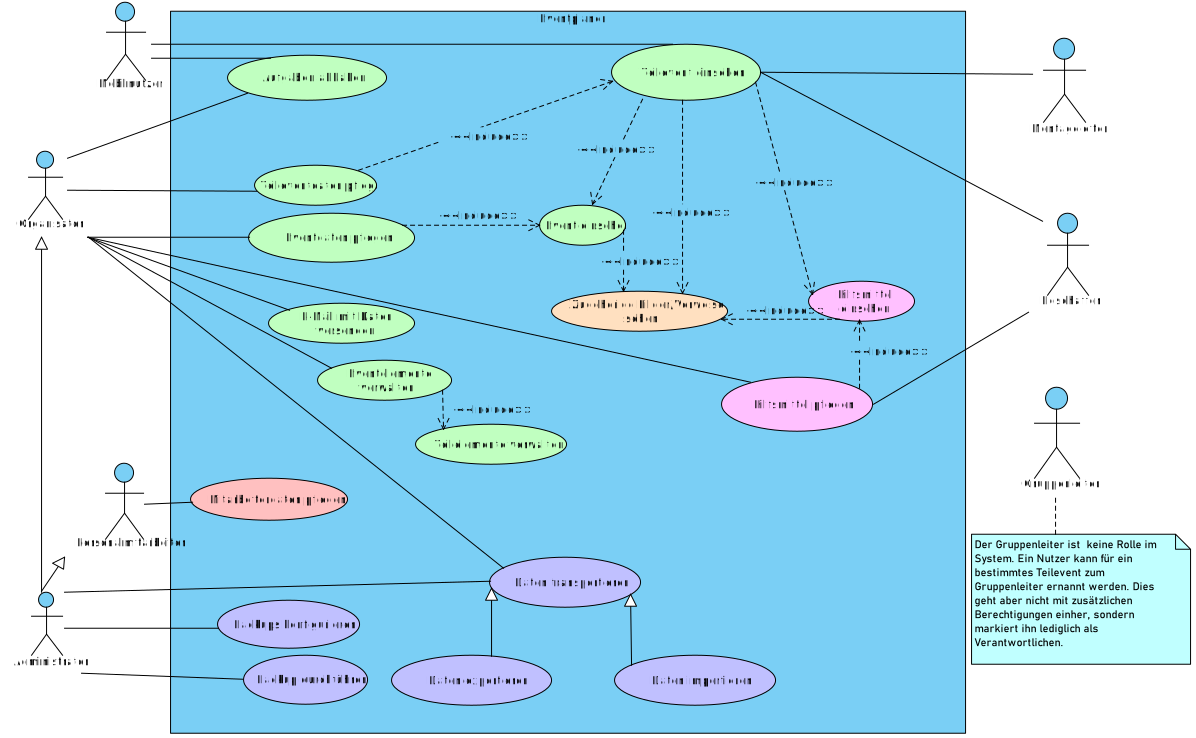
\includegraphics[width=0.98\columnwidth]{Bilder/use-case-diagramm-grob.pdf}
    \caption{Use-Case-Diagramm der gesamten Anwendung}
    \label{fig:uc:grob}
\end{figure}
Abbildung ~\ref{fig:uc:grob} zeigt die Use-Cases der gesamten Anwendung. Verschiedene Farben kennzeichnen die verschiedenen Themengebiete. Zuerst werden alle Use-Cases grob dargestellt und beschrieben sowie deren Zusammenhänge gezeigt.

\section{Erläuterung der Akteure}
Der Eventplaner besitzt fünf Rollen, die Nutzern zugewiesen werden können. Der Gruppenleiter und Mobilnutzer sind keine dem Nutzer zuweisbare Rollen. Durch die zugewiesene Rolle wird festgelegt, welche Zugriffsrechte ein Nutzer im System hat. Im Folgenden soll jeder in den Diagrammen auftauchende Akteur kurz erläutert werden. Es wird immer nur die männliche Formulierung der Rolle für alle Geschlechter verwendet.

\paragraph{Montageleiter}
Der Montageleiter hat lesenden Zugriff auf seinen Arbeitsbereich betreffende Objekte. Aus der Analyse ergibt sich, dass dieses die ihm zugewiesenen Teilevents sowie alle darüberstehenden Teilevents und Events sind. Damit kann der Montageleiter auch die dem Teilevent zugewiesenen Hilfsmittel, Bilder und Verweise betrachten. 

Zu beachten ist, dass der Montageleiter, auch wenn er für das Teilevent verantwortlich ist, es nicht als abgeschlossen markieren kann. Aus der Analyse ergibt sich, dass das durch einen Anruf an den Organisator geschieht, welcher es dann im System einträgt. Des Weiteren kann der Montageleiter keine Veränderungen an der Verantwortlichkeit des Teilevents tätigen. Ist dieser zum Beispiel auch der Gruppenleiter des Projektes und meldet sich eine weitere freiwillige Person, die helfen möchte, muss auch hier der Organisator diese eintragen.

\paragraph{Beschaffer}
Das Beschaffungspersonal besorgt und verwaltet Hilfsmittel. Dafür hat es Zugriff auf die zugewiesenen Teilevents, die übergeordneten Teilevents und Events, sowie zugewiesenen Hilfsmittel, Bilder und Verweise. Des Weiteren hat das Beschaffungspersonal aber auch noch Zugriff darauf, Hilfsmittel zu verwalten. 

Dadurch sollen Organisatoren davon entlastet werden, die genauen Details der Hilfsmittel zu verwalten. Trotzdem müssen auch Beschaffer dem Organisator manuell mitteilen, dass eine Aufgabe erledigt ist und abgehakt werden kann.

\paragraph{Administrator}
Der Administrator hat Zugriff auf jegliche Funktionalität. Er ist der einzige Akteur, der ein Backup ausführen kann und die automatischen wöchtenlichen Backups konfigurieren kann.

\paragraph{Personalmitarbeiter}
Der Personalmitarbeiter nutzt das System nur, um die Mitarbeiterdaten zu verwalten. Er benötigt keine Funktionalität, die mit dem Kerngeschäft der Eventplanung zu tun hat, da sein Aufgabenbereich nicht das Kerngeschäft beinhaltet.

\paragraph{Organisator}
Der Organisator hat als Leiter und Planer von Events die meisten Rechte. Er kann Events planen und somit auch alle Daten dazu, sowie zu untergeordneten Teilevents einsehen. Er kann diese Daten jedoch nicht nur einsehen, sondern auch in jeder Weise bearbeiten. Des Weiteren können Organisatoren E-Mails mit Informationen an Personen senden, die es betrifft sowie ausführliche Daten-Exporte und -Importe durchführen.

Eine wichtige Aufgabe des Organisators ist es, während der Durchführung eines Events die einzelnen Teilevents abzuhaken, sobald Mitarbeiter mitteilen mit einer Aufgabe fertig zu sein.

\paragraph{Mobilnutzer}
Der Mobilnutzer ist in diesem Konzept eine Person vor Ort, die entweder Informationen zu dem ihr zugewiesenen Teilevent einsehen möchte oder eines der zugewiesenen Teilevents abhaken möchte. Der Mobilnutzer kann somit ihm zugewiesene Teilevents einsehen, sowie die zugehörigen Daten. Auch kann dieser ihm direkt zugewiesene Teilevents als fertig markieren. Das ermöglicht es, ein Teilevent abzuschließen, ohne dass der Organisator involviert wird.

Der Mobilnutzer ist somit keine Rolle, die einem durch den Personalmitarbeiter zugewiesen wird, sondern man implizit ausübt, wenn durch die Mobilversion auf das System zugegriffen wird.

\paragraph{Gruppenleiter}
Der Gruppenleiter ist keine Rolle im System, die von einem Personalmitarbeiter einem Nutzer zugewiesen wird. Ein Mitarbeiter kann für ein bestimmtes Teilevent zum Gruppenleiter ernannt werden. Dieses gibt ihm keine weiteren Berechtigungen, aber markiert ihn als Verantwortlichen für dieses Teilevent.

\section{Erläuterung der Use-Cases}

\paragraph{Zugehörige Bilder sehen}
Ein wesentliches Feature der Software ist die Möglichkeit, verschiedensten Elementen wie Events oder Hilfsmitteln Bilder zuzuordnen. Diese im Nachhinein dann einsehen zu können, ist darum ein integraler Use-Case für den Eventplaner, welcher darum auch in einigen anderen Use-Cases verwendet wird.

\paragraph{Hilfsmittel einsehen}
Zur Planung und Durchführung von Events ist eine Vielzahl sogenannter Hilfsmittel notwendig. Dies können beispielsweise Kerzen bei einer Hochzeit oder Stühle und Tische für einen Kongress sein. Als Teil vieler anderer Use-Cases müssen diese eingesehen beziehungsweise gefiltert und durchsucht werden können.

\paragraph{Hilfsmittel pflegen}
Dieser Use-Case betrifft die Verwaltung der Hilfsmittel unabhängig von bestimmten Events. Er umfasst beispielsweise Funktionalitäten wie das Hinzufügen und entfernen von Hilfsmitteln aus der Datenbasis oder das pflegen der Lagerbestände. Dieser Use-Case ist nur Benutzern mit den Rollen \enquote{Beschaffer} oder \enquote{Organisator} zugänglich.

\paragraph{Teilevent einsehen}
Dieser Use-Case dient dem Einsehen der Daten eines Teilevents. Er setzt sich aus mehreren weiteren Use-Cases zusammen: Da der Nutzer das gewünschte Teilevent auch im Kontext des Übergeordneten Events betrachten können soll, beinhaltet dieser Use-Case auch das \enquote{Event einsehen}. Da einem Teilevent auch Bilder zugeordnet werden können, ist auch der Use-Case \enquote{Zugehörige Bilder sehen} Teil dieses Use-Cases. Ein weiterer wichtiger Bestandteil sind die Hilfsmittel eines Teilevents.

\paragraph{Teileventdaten pflegen}
Jedes Teilevent besitzt eine Vielzahl von Attributen. Diese können sowohl primitiv wie Name und Beschreibung als auch Assoziationen zu anderen Elementen wie beispielweise den Hilfsmitteln oder untergeordneten Teilevents sein. Diese müssen durch die Organisatoren bearbeitet werden können. Handelt es sich um Assoziationen, so soll die Auswahl möglichst mittels Auswahllisten erfolgen. Selbstverständlich umfasst dieser Use-Case auch das \enquote{Teilevent einsehen}.

\paragraph{Event einsehen}
Zur Verrichtung ihrer Tätigkeiten müssen Nutzer die Möglichkeit haben, die Daten der Events einzusehen. Dieses umfasst neben primitiven Attributen und Assoziationen auch das Einsehen der zugehörigen Bilder.

\paragraph{Eventdaten pflegen}
Analog zu den Attributen eines Teilevents müssen auch die Attribute der übergeordneten Events bearbeitet werden können. Dieses umfasst auch das \enquote{Event einsehen}. Auch dieser Use-Case ist lediglich den Organisatoren zugänglich.

\paragraph{E-Mail mit Daten versenden}
Zur besseren Kommunikation mit anderen Beteiligten haben Organisatoren die Möglichkeit E-Mails mit Daten eines Events oder Teilevents zu versenden. Diese werden durch die Software automatisch generiert und dann im Standardmailclient des verwendeten Endgeräts sendebreit geöffnet.

\paragraph{Mitarbeiterdaten pflegen}
Um die Mitarbeiter adäquat zu bestimmten Teilevents zuordnen zu können müssen bestimmte Informationen über die Mitarbeiter in der Software erfasst und ggf. geändert werden können. Diese Aufgabe und somit auch dieser Use-Case obliegt allein den Personalmitarbeitern.

\paragraph{Daten exportieren}
Die in der Software verwalteten Daten können in Form von CSV-Dateien exportiert werden. Hierbei hat der Nutzer die Möglichkeit, die zu exportierenden Daten nach den Attributen der gewünschten Objekte zu filtern.

\paragraph{Daten importierten}
Analog zum Expotieren von Daten ist auch ein Import von Daten aus CSV-Dateien möglich und auch hier hat der Nutzer die Möglichkeit, bevor er den Import ausführt die zu importierenden Daten nach deren Attributen zu filtern.

\paragraph{Daten transportieren}
Dieser Use-Case fasst die beinden ihm untergeordneten Use-Cases \enquote{Daten exportieren} und \enquote{Daten importieren} zusammen. Er ist, außer natürlich dem Administrator, lediglich den Organisatoren zugänglich.

\paragraph{Backups konfigurieren}
Der Administrator hat die Möglichkeit durch das System automatisch durchzuführende Backups zu konfigurieren. Dieser Use-Case umfasst das Festlegen des Zielverzeichnisses, in welchem die gesicherten Daten gespeichert werden sollen, sowie den Zeitpunkt, zu dem das Backup ausgeführt werden soll.

\paragraph{Backups durchführen}
Neben den automatischen Backups bietet das System auch die Möglichkeit, Backups manuell durchzuführen. Allerdings steht auch dieser Use-Case nur dem Administrator zur Verfügung.

\paragraph{Aufgaben abhaken}
Das Abhaken von Aufgaben ist ein Use-Case, welcher erst in der zweiten Ausbaustufe der Software von Interesse sein wird. Hier muss es dem Nutzer möglich sein, erledigte Aufgaben mittels einer Mobile-App abzuhaken, also als abgeschlossen zu markieren.

\section{Verfeinerung des Use-Case \enquote{Teileventdaten pflegen}}
\begin{figure}[ht!]
    \centering
    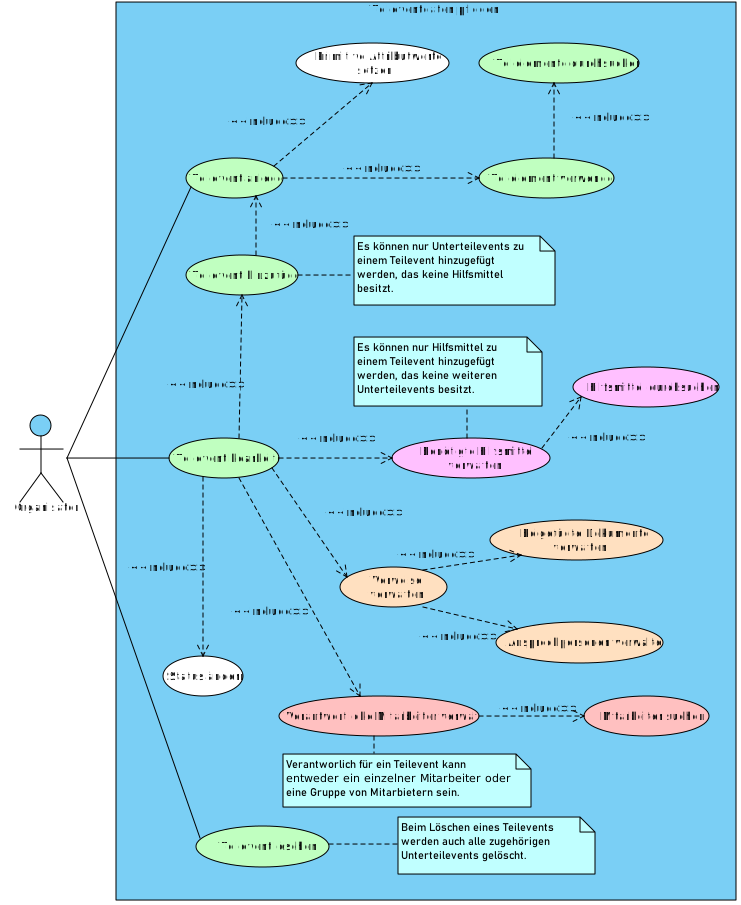
\includegraphics[width=0.98\columnwidth]{Bilder/use-case-diagramm-fein.pdf}
    \caption{Use-Case-Diagramm des Use-Case \enquote{Teileventdaten pflegen}}
    \label{fig:uc:fein}
\end{figure}

\paragraph{Teilelemente durchsuchen}
Die vorhandenen Teilelemente können durch Freitext durchsucht werden. Der Suchtext wird mit den Attributen des Teilelements verglichen und bei Übereinstimmung in der Ergebnisliste angezeigt. Dieses dient dazu, den Nutzer dabei zu unterstützen schnell die korrekten Teilelemente zu finden, um diese auswählen zu können.

\paragraph{Teilelement verwenden}
Es kann ein vorgefertigtes Teilelement als Vorlage für ein neues Teilevent verwendet werden. Dadurch kann die bereits bei anderen Events getane Arbeit wiederverwendet werden. Trotzdem müssen dann noch die primitiven Attribute vervollständigt werden.

\paragraph{Primitive Attribute setzen}
Beim Anlegen müssen die primitiven Attribute eines Teilevents gesetzt werden. Dazu gehören unter Anderem der Name, die Start- und Endtermine und die Beschreibung. Dadurch hat jedes Teilevent direkt nach dem Anlegen schon grundlegende Informationen und kann so weiterverwendet werden.

\paragraph{Teilevent anlegen}
Es können neue Teilevents angelegt werden. Dafür kann entweder ein Teilelement als Vorlage verwendet werden oder blank begonnen werden. Beim Anlegen werden die primitiven Attribute gesetzt und sobald dieses geschehen ist, kann angefangen werden, die weiteren Attribute und zugehörigen Objekte zu verwalten.

\paragraph{Teilevent hinzufügen}
Zu einem bestehenden Teilevent können Unterteilevents hinzugefügt werden. Dieses Teilevent stellt dann keine konkrete Aktion dar, die durchgeführt werden soll, sondern eine logische Gruppierung von Teilevents, die wiederum Gruppen an Aktionen sein könnten. Wird ein Unterteilevent hinzugefügt, so können diesem Teilevent keine Hilfsmittel hinzugefügt werden. Um ein Unterteilevent hinzuzufügen, muss dieses Unterteilevent dafür grundsätzlich neu angelegt werden.

\paragraph{Hilfsmittel durchsuchen}
Hilfsmittel können anhand einer Freitextsuche gefiltert werden. Der Suchtext wird dann mit den Attributen verglichen und bei Übereinstimmung wird das Hilfsmittel in der Ergebnisliste angezeigt. Dieses dient der Benutzerfreundlichkeit, da das Eventplanungsunternehmen eine große Basis an Hilfsmitteln hat, die nicht manuell komplett durchsucht werden soll.

\paragraph{Benötigte Hilfsmittel verwalten}
Ein Teilevent, welches keine Unterteilevents hat, stellt eine Aktion dar, die ausgeführt werden soll. Daher können diesem Teilevent Hilfsmittel zugeordnet werden, die zur Durchführung benötigt werden oder diese unterstützen. Hilfsmittel die einem Teilevent zugeordnet sind, sind für den Zeitraum des Teilevents gebucht. Die Zuordnung eines Hilfsmittel geschieht durch eine Suche mit anschließender Auswahl.

\paragraph{Beigefügte Dokumente verwalten}
Einem Verweis können beliebige Dokumente zugeordnet werden. Diese werden in dem Verzeichnis der zentralen Datenbasis abgelegt. In diesem Use-Case können diese Dokumente angelegt oder gelöscht werden. Ein Beispiel dafür wäre der Mietvertrag der Location eines Events, dadurch kann auch dieser im System verwaltet werden und geht nicht verloren.

\paragraph{Ansprechpersonen verwalten}
Einem Verweis können beliebig viele Ansprechpersonen zugeordnet werden, diese halten jeweils die Kontaktdaten dieser Person für zukünftige Zwecke fest. Ein Beispiel für eine Ansprechperson wäre der Hausmeister der Halle, die für ein Konzert verwendet wird. In diesem Use-Case können dann neue Ansprechpersonen angelegt, vorhandene bearbeitet oder gelöscht werden.

\paragraph{Verweise verwalten}
Zu jedem Teilevent können beliebig viele Verweise angelegt werden. In dem Verweis ist optional ein Firmenname eingetragen und dem Verweis können Dokumente und Ansprechpersonen zugeordnet werden.

\paragraph{Mitarbeiter suchen}
Mitarbeiter können in einer Freitextsuche gefunden werden. Der Freitext wird mit allen Attributen des Mitarbeiters verglichen und zutreffende Mitarbeiter in einer Ergebnisliste angezeigt. Dieses wird hier dafür verwendet, die Mitarbeiter für die Zuweisung der Verantwortlichkeit auszusuchen.

\paragraph{Verantwortliche Mitarbeiter verwalten}
Die Verantwortlichkeit für ein Teilevent kann bei der Bearbeitung festgelegt werden. Wird beim Erstellen keine Verantwortlichkeit festgelegt, so ist der Ersteller standardmäßig verantwortlich. Es kann ein einzelner Mitarbeiter oder eine Gruppe an Mitarbeitern als verantwortlich markiert werden. Wird eine Gruppe als verantwortlich markiert, muss einer der Mitarbeiter als Gruppenleiter markiert werden. Die Mitarbeiter werden durch eine Suche ausgewählt.

\paragraph{Status ändern}
Der Status eines Teilevents kann geändert werden. Dabei wird aus einer Auswahlliste einer der möglichen vordefinierten Status ausgewählt. Dieses ist eine Veränderung eines primitiven Attributes. Durch diese Funktionalität kann der Organisator zum Beispiel Aufgaben abhaken, sobald sie ihm als erledigt gemeldet werden oder als \enquote{geplant} markieren, um eine Übersicht darüber zu haben, was er bereits fertig geplant hat.

\paragraph{Teilevent bearbeiten}
Ein Teilevent kann nach der Erstellung immer noch bearbeitet werden. Dabei können alle primitiven Attribute verändert und zugehörige Objekte verwaltet werden. Dieses ermöglicht es, das Teilevent nachträglich noch zu ändern, falls sich die Umstände ändern oder bei der Planung Fehler geschehen sind.

\paragraph{Teilevent löschen}
Sollte ein Teilevent als unnötig angesehen werden, soll natürlich die Möglichkeit bestehen, dieses zu löschen. Wird es gelöscht, so müssen kaskadierend auch alle Unterteilevents des Teilevents gelöscht werden, da ein Teilevent nicht ohne Ober(teil)event existieren kann.

